\chapter{Architecture}

A high level abstraction of the general architecture of the system is available \autoref{fig:Architecture}.
The system is composed from 3 principles building block:
\begin{itemize}
    \item \textbf{DingNet simulator} $\rightarrow$ represent the LoRaWan network where are presents both sensors and gateway and it simulates the communication between this two kinds of network entities.
    \item \textbf{MQTT broker} $\rightarrow$ intermediary between the LoRaWan network and AC program.
    \item \textbf{Protelis MQTT back-end} $\rightarrow$ entry point of Protelis program. The back-end hides the real network topology, so the Protelis program can use a logical proximity based network. In this case the communication will be based on MQTT.
    \item \textbf{Protelis program} $\rightarrow$ the aggregate program that identifies areas with good air quality and defines the required routes
\end{itemize}

\begin{figure}[h]
    \centering
    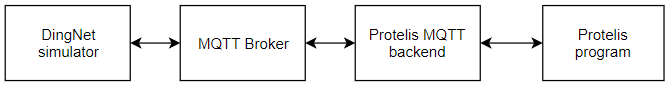
\includegraphics{DingNet_en.png}
    \caption{System architecture}
    \label{fig:Architecture}
\end{figure}